\documentclass[preview]{standalone}

\usepackage{amsmath}
\usepackage{amssymb}
\usepackage{bettelini}
\usepackage{stellar}
\usepackage{definitions}

\begin{document}

\id{measuretheory-lebesgue-spaces-completeness}
\genpage

\section{Completeness of L1}

\begin{snippettheorem}{normed-space-completeness-absolute-series-criterion}{Absolute-series criterion for completeness}
    A normed vector space \((X,\|\cdot\|)\) is complete if and only if every
    series \(\sum_nx_n\) satisfying
    \[
        \sum_{n=1}^{\infty}\|x_n\|<+\infty
    \]
    converges in \(X\).
\end{snippettheorem}

\begin{snippetproof}{normed-space-completeness-absolute-series-criterion-proof}{normed-space-completeness-absolute-series-criterion}{Absolute-series criterion for completeness}
    \begin{iffproof}
        \item Suppose that \(X\) is complete and
            \(\sum_n\|x_n\|<+\infty\). For the partial sums
            \(s_N=\sum_{n=1}^Nx_n\) and \(M>N\),
            \[
                \|s_M-s_N\|
                =\left\|\sum_{n=N+1}^Mx_n\right\|
                \leq\sum_{n=N+1}^M\|x_n\|.
            \]
            The numerical tails tend to zero, so \(\{s_N\}\) is Cauchy and
            therefore converges in \(X\).
        \item Suppose that every absolutely convergent series converges, and
            let \(\{x_n\}\) be Cauchy. Choose a subsequence
            \(\{x_{n_k}\}\) such that
            \[
                \|x_{n_{k+1}}-x_{n_k}\|<2^{-k}.
            \]
            The series
            \[
                \sum_{k=1}^{\infty}(x_{n_{k+1}}-x_{n_k})
            \]
            converges absolutely and hence converges in \(X\). Its
            telescoping partial sums show that \(x_{n_k}\to x\) for some
            \(x\in X\). A Cauchy sequence with a convergent subsequence
            converges to the same limit, so \(x_n\to x\).
    \end{iffproof}
\end{snippetproof}

\begin{snippettheorem}{l-one-space-banach-theorem}{\(L^1\) is a Banach space}
    For every measure space \((X,\mathcal M,\mu)\), the normed space
    \((L^1(\mu),\|\cdot\|_1)\) is complete.
\end{snippettheorem}

\begin{snippetproof}{l-one-space-banach-theorem-proof}{l-one-space-banach-theorem}{\(L^1\) is a Banach space}
    By the absolute-series criterion, it is enough to consider
    \(\{f_n\}\subseteq L^1(\mu)\) such that
    \[
        \sum_{n=1}^{\infty}\|f_n\|_1
        =\sum_{n=1}^{\infty}\int_X|f_n|\,d\mu<+\infty.
    \]
    The integration theorem for absolutely summable series gives a function
    \(f\in L^1(\mu)\) such that \(\sum_nf_n=f\) almost everywhere. If
    \[
        \varphi=\sum_{n=1}^{\infty}|f_n|\in L^1(\mu),
    \]
    then, for the partial sums \(S_k\),
    \[
        |S_k-f|\leq2\varphi
    \]
    and \(S_k\to f\) almost everywhere. Dominated convergence yields
    \[
        \|S_k-f\|_1
        =\int_X|S_k-f|\,d\mu\longrightarrow0.
    \]
    Thus every absolutely convergent series converges in \(L^1(\mu)\).
\end{snippetproof}

\begin{snippet}{dominated-convergence-as-l-one-convergence}
    Dominated convergence can be read as a norm-convergence theorem: if
    \(f_n\to f\) almost everywhere and \(|f_n|\leq g\in L^1\), then
    \[
        \|f_n-f\|_1\longrightarrow0.
    \]
    The existence of a common dominator is a sufficient condition, not a
    necessary one for \(L^1\)-convergence.
\end{snippet}

\begin{snippetexample}{typewriter-sequence-example}{The typewriter sequence}
    \begin{center}
        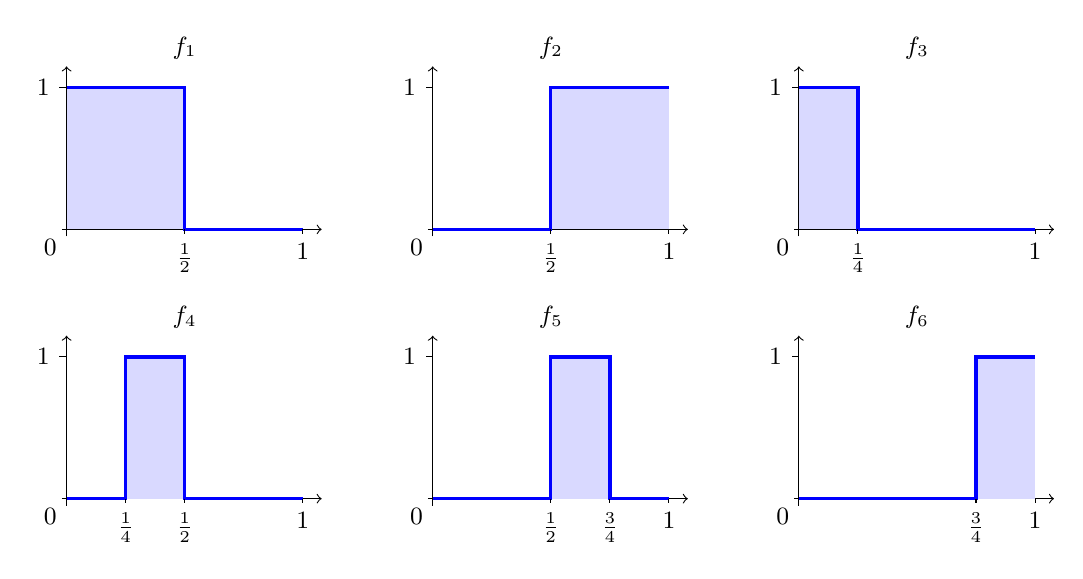
\begin{tikzpicture}[x=3cm,y=1.8cm,every node/.style={font=\small}]
            \begin{scope}[shift={(0,0)}]
                \draw[->] (-0.02,0) -- (1.08,0);
                \draw[->] (0,-0.05) -- (0,1.15);
                \fill[blue!15] (0,0) rectangle (0.5,1);
                \draw[very thick,blue] (0,1) -- (0.5,1) -- (0.5,0) -- (1,0);
                \draw (0,1) -- (-0.03,1) node[left] {$1$};
                \draw (0.5,0) -- (0.5,-0.03) node[below] {$\frac12$};
                \draw (1,0) -- (1,-0.03) node[below] {$1$};
                \node[below left] at (0,0) {$0$};
                \node at (0.5,1.28) {$f_1$};
            \end{scope}

            \begin{scope}[shift={(1.55,0)}]
                \draw[->] (-0.02,0) -- (1.08,0);
                \draw[->] (0,-0.05) -- (0,1.15);
                \fill[blue!15] (0.5,0) rectangle (1,1);
                \draw[very thick,blue] (0,0) -- (0.5,0) -- (0.5,1) -- (1,1);
                \draw (0,1) -- (-0.03,1) node[left] {$1$};
                \draw (0.5,0) -- (0.5,-0.03) node[below] {$\frac12$};
                \draw (1,0) -- (1,-0.03) node[below] {$1$};
                \node[below left] at (0,0) {$0$};
                \node at (0.5,1.28) {$f_2$};
            \end{scope}

            \begin{scope}[shift={(3.1,0)}]
                \draw[->] (-0.02,0) -- (1.08,0);
                \draw[->] (0,-0.05) -- (0,1.15);
                \fill[blue!15] (0,0) rectangle (0.25,1);
                \draw[very thick,blue] (0,1) -- (0.25,1) -- (0.25,0) -- (1,0);
                \draw (0,1) -- (-0.03,1) node[left] {$1$};
                \draw (0.25,0) -- (0.25,-0.03) node[below] {$\frac14$};
                \draw (1,0) -- (1,-0.03) node[below] {$1$};
                \node[below left] at (0,0) {$0$};
                \node at (0.5,1.28) {$f_3$};
            \end{scope}

            \begin{scope}[shift={(0,-1.9)}]
                \draw[->] (-0.02,0) -- (1.08,0);
                \draw[->] (0,-0.05) -- (0,1.15);
                \fill[blue!15] (0.25,0) rectangle (0.5,1);
                \draw[very thick,blue] (0,0) -- (0.25,0) -- (0.25,1) -- (0.5,1) -- (0.5,0) -- (1,0);
                \draw (0,1) -- (-0.03,1) node[left] {$1$};
                \draw (0.25,0) -- (0.25,-0.03) node[below] {$\frac14$};
                \draw (0.5,0) -- (0.5,-0.03) node[below] {$\frac12$};
                \draw (1,0) -- (1,-0.03) node[below] {$1$};
                \node[below left] at (0,0) {$0$};
                \node at (0.5,1.28) {$f_4$};
            \end{scope}

            \begin{scope}[shift={(1.55,-1.9)}]
                \draw[->] (-0.02,0) -- (1.08,0);
                \draw[->] (0,-0.05) -- (0,1.15);
                \fill[blue!15] (0.5,0) rectangle (0.75,1);
                \draw[very thick,blue] (0,0) -- (0.5,0) -- (0.5,1) -- (0.75,1) -- (0.75,0) -- (1,0);
                \draw (0,1) -- (-0.03,1) node[left] {$1$};
                \draw (0.5,0) -- (0.5,-0.03) node[below] {$\frac12$};
                \draw (0.75,0) -- (0.75,-0.03) node[below] {$\frac34$};
                \draw (1,0) -- (1,-0.03) node[below] {$1$};
                \node[below left] at (0,0) {$0$};
                \node at (0.5,1.28) {$f_5$};
            \end{scope}

            \begin{scope}[shift={(3.1,-1.9)}]
                \draw[->] (-0.02,0) -- (1.08,0);
                \draw[->] (0,-0.05) -- (0,1.15);
                \fill[blue!15] (0.75,0) rectangle (1,1);
                \draw[very thick,blue] (0,0) -- (0.75,0) -- (0.75,1) -- (1,1);
                \draw (0,1) -- (-0.03,1) node[left] {$1$};
                \draw (0.75,0) -- (0.75,-0.03) node[below] {$\frac34$};
                \draw (1,0) -- (1,-0.03) node[below] {$1$};
                \node[below left] at (0,0) {$0$};
                \node at (0.5,1.28) {$f_6$};
            \end{scope}
        \end{tikzpicture}
    \end{center}
    Enumerate the dyadic intervals level by level and let \(f_n\) be their
    indicator functions, as in the figure. Their lengths tend to zero, so
    \(f_n\to0\) in \(L^1([0,1])\). Nevertheless, almost every point belongs
    to one interval at every dyadic level and also lies outside infinitely
    many listed intervals. Thus the sequence does not converge pointwise
    almost everywhere. It has subsequences converging almost everywhere to
    zero, but no almost-everywhere convergent subsequence can have a different
    limit.
\end{snippetexample}

\end{document}
